\documentclass{article}

\usepackage{graphicx}
\usepackage{tikz}
\usepackage{tikzsymbols}
\usetikzlibrary{calc,patterns,shapes.geometric}
\pagestyle{empty}
\usepackage[margin=0pt]{geometry}
\geometry{papersize={14in,12in}}

\def\centerarc[#1](#2)(#3:#4:#5){\draw[#1] ($(#2)+({#5*cos(#3)},{#5*sin(#3)})$) arc (#3:#4:#5);}

\begin{document}
	\begin{figure}
		\centering
		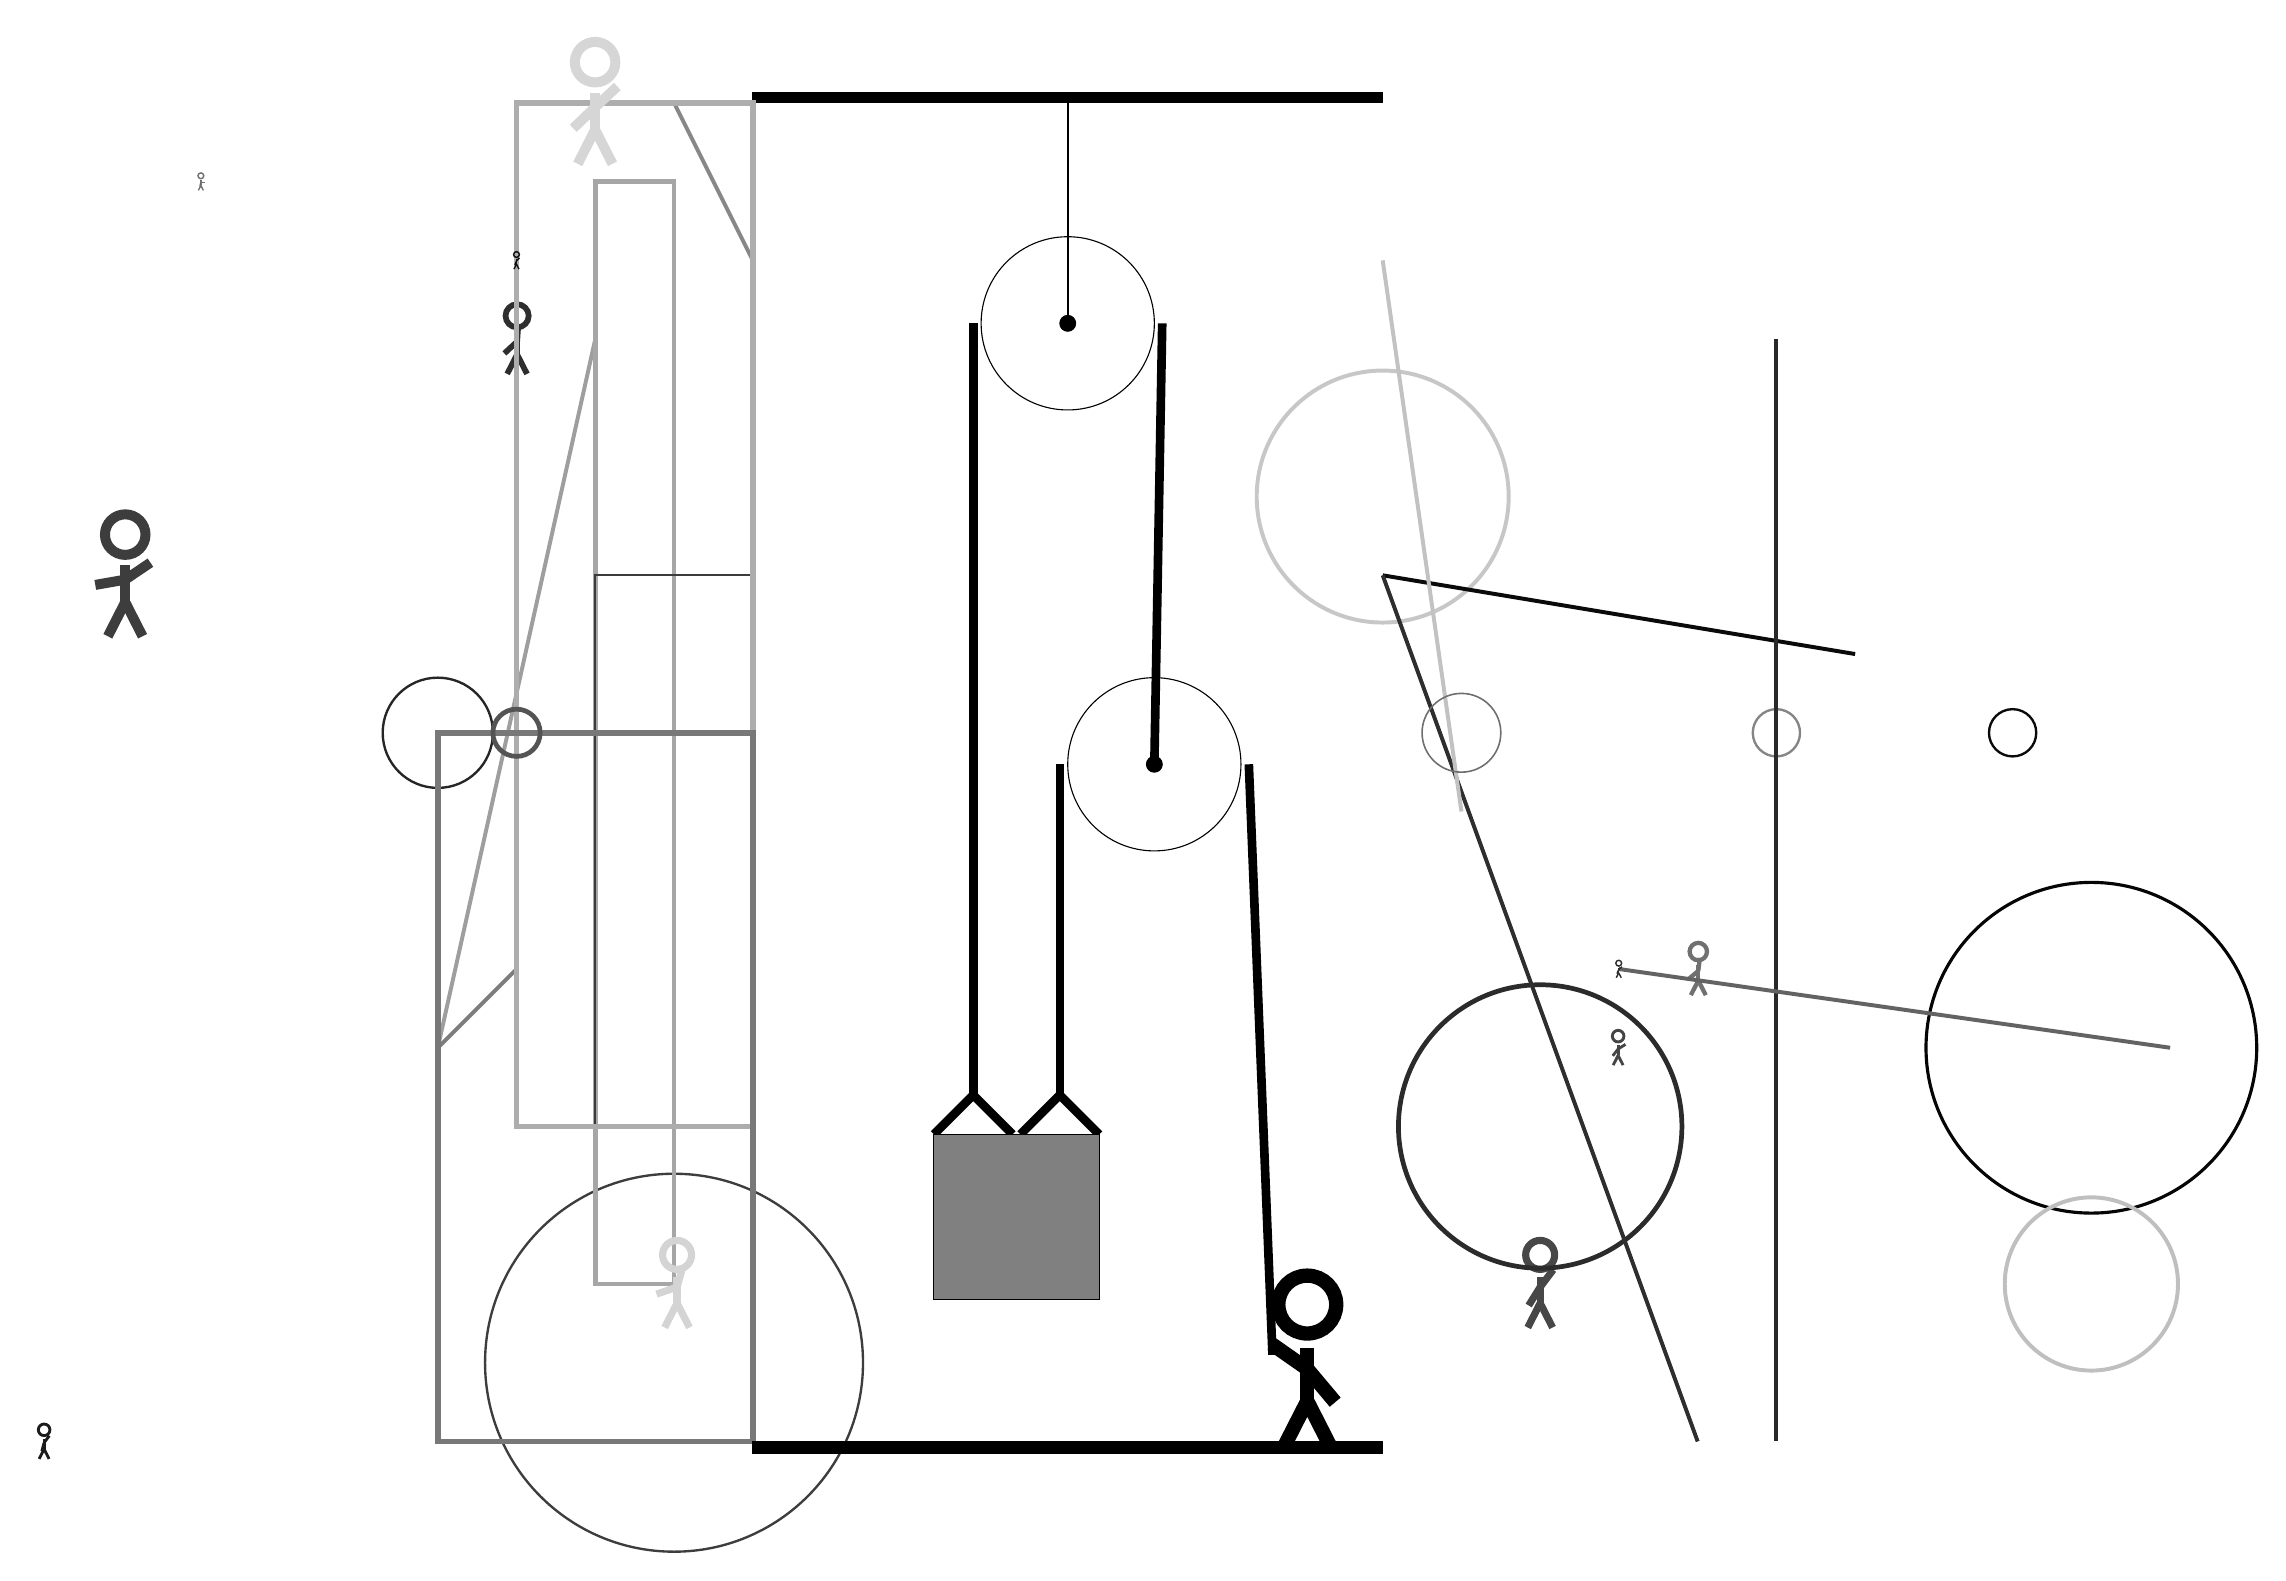
\begin{tikzpicture}
			%%%%% START %%%%%
			
			\draw[fill=black] (-2, 14) rectangle (6, 14.125);
			
			\draw [line width=0.4mm, color=black!98](15, 2) circle (2.1);
			
			\node[line width=0.4mm, color=black!72] at (8, -1) {\Strichmaxerl[5][58][53]};
			\node[line width=0.4mm, color=black!56] at (-9, 13) {\Strichmaxerl[1][77][0]};
			\node[line width=0.5mm, color=black!56] at (10, 3) {\Strichmaxerl[3][40][83]};
			
			\draw [line width=0.5mm, color=black!22](6, 9) circle (1.6);
			
			\draw [line width=0.3mm, color=black!76](-3, -2) circle (2.4);
			\draw [line width=0.3mm, color=black!48](11, 6) circle (0.3);
			\draw[line width=0.5mm, color=black!96](6, 8) -- (12, 7);
			\draw [line width=0.3mm, color=black!96](14, 6) circle (0.3);
			\draw[line width=0.5mm, color=black!38](-4, 11) -- (-6, 2);
			\draw [line width=0.5mm, color=black!25](15, -1) circle (1.1);
			\draw[line width=0.5mm, color=black!84](11, 11) -- (11, -3);
			\node[line width=0.6mm, color=black!76] at (-10, 8) {\Strichmaxerl[7][10][34]};
			\draw [line width=0.6mm, color=black!83](8, 1) circle (1.8);
			\draw[line width=0.5mm, color=black!51](-6, 2) -- (-5, 3);
			\draw[line width=0.6mm, color=black!35] (-3, -1) rectangle (-4, 13);
			\draw[line width=0.5mm, color=black!82](10, -3) -- (6, 8);
			\node[line width=0.5mm, color=black!82] at (-5, 11) {\Strichmaxerl[4][43][86]};
			\draw[line width=0.5mm, color=black!61](9, 3) -- (16, 2);
			\node[line width=0.4mm, color=black!89] at (-11, -3) {\Strichmaxerl[2][75][53]};
			\node[line width=0.7mm, color=black!82] at (9, 3) {\Strichmaxerl[1][66][41]};
			
			\node[line width=0.4mm, color=black!73] at (9, 2) {\Strichmaxerl[2][52][32]};
			\node[line width=0.5mm, color=black!17] at (-3, -1) {\Strichmaxerl[5][19][74]};
			\draw[line width=0.5mm, color=black!24](7, 5) -- (6, 12);
			\draw[line width=0.5mm, color=black!47](-2, 12) -- (-3, 14);
			\draw[line width=0.3mm, color=black!77] (-4, 8) rectangle (-2, 1);
			\draw [line width=0.3mm, color=black!85](-6, 6) circle (0.7);
			\draw[line width=0.7mm, color=black!32] (-2, 14) rectangle (-5, 1);
			\draw [line width=0.2mm, color=black!57](7, 6) circle (0.5);
			\node[line width=0.5mm, color=black!16] at (-4, 14) {\Strichmaxerl[7][44][43]};
			\node[line width=0.3mm, color=black!94] at (-5, 12) {\Strichmaxerl[1][68][46]};
			
			\draw[line width=0.7mm, color=black!53] (-2, -3) rectangle (-6, 6);
			\draw [line width=0.6mm, color=black!67](-5, 6) circle (0.3);
			
			
			\draw (2, 11.2) circle (1.1);
			\draw[fill=black] (2, 11.2) circle (0.1);
			\draw[thick] (2, 11.2) -- (2, 14);
			
			\draw (3.1, 5.6) circle (1.1);
			\draw[fill=black] (3.1, 5.6) circle (0.1);
			
			\draw[line width = 1.1mm]  (0.3, 0.9) -- (0.8, 1.4) -- (1.3, 0.9);
			\draw[line width = 1.1mm]  (1.4, 0.9) -- (1.9, 1.4) -- (2.4, 0.9);
			\draw[fill=black!50] (0.3, 0.9) rectangle (2.4, -1.2);
			
			\draw[line width = 1.1mm] (0.8, 11.2) -- (0.8, 1.4);
			\centerarc[line width = 1.1mm](2, 11.2)(0:180:1.2000000000000002);
			\draw[line width = 1.1mm] (3.2, 11.2) -- (3.1, 5.6);
			\draw[line width = 1.1mm] (1.9, 5.6) -- (1.9, 1.4);
			\centerarc[line width = 1.1mm](3.1, 5.6)(0:180:1.2000000000000002);
			\draw[line width = 1.1mm] (4.3, 5.6) -- (4.6, -1.9);
			
			\node at (5, -2) {\Strichmaxerl[10][-35][-50]};
			
			\draw[fill=black] (-2, -3) rectangle (6, -3.15);
			
			%%%%% END %%%%%
		\end{tikzpicture}
	\end{figure}	
\end{document}